\chapter{Matching in General Graphs}
Here we give a similar algorithm for finding maximum matching in general graph as in the case of bipartite graphs in \autoref{section:bp-augment-path}. We will give a similar characterization for the maximum matching in general graphs. We have already showed \hyperref[th:bergesthm]{Berge's Lemma} that a matching $M$ is maximum if and only if there are no $M$-augmenting paths in $G$. So we will search for augmenting paths in the graph $G$ with respect to a matching $M$.
\section{Flowers and Blossoms}
By the above theorem like in the case of bipartite graphs we will search for augmenting paths in $G$ for matching $M$ and if we can find an augmenting path $p$ we will update the matching by taking $M'=M\triangle p$ and obtain a larger matching. But unlike bipartite graphs we can not run the same algorithm for finding augmenting paths as there can be edges between two odd layers or two even layers. So in the $M$-alternating tree there can be odd cycles, but these odd cycles have all vertices except one vertex are matched using edges of the cycle. So we look for these special structures in the $M$-alternating tree called \emph{blossom} and \emph{flower}.
\begin{Definition}{Flower and Blossom}{}
	\begin{minipage}{0.65\textwidth}
		For a matching $M$ a \emph{flower} consists of an even $M$-alternating path $P$ from an exposed vertex $u$ to vertex $v$, called the \emph{stem} and an odd cycle containing $v$ in which the edges alternate between in and out of the matching except for the two edges incident to $v$. This odd cycle is called the \emph{blossom}.
	\end{minipage}\hspace{5pt}
	\begin{minipage}{0.25\textwidth}
		\usetikzlibrary{decorations.pathreplacing,arrows.meta, calc}
		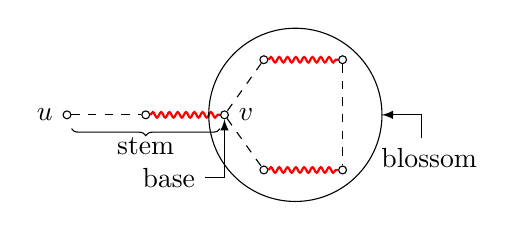
\begin{tikzpicture}[
				vertex/.style={circle, draw, inner sep=0pt, minimum size=1mm},
			]
			\node[vertex, label=left:{$u$}] (u) at (0,0) {};
			\node[vertex] (a) at (1,0) {};
			\node[vertex, label=right:{$v$}] (v) at (2,0) {};
			\node[vertex] (c1) at (2.5,0.7) {};
			\node[vertex] (c2) at (3.5,0.7) {};
			\node[vertex] (c3) at (3.5,-0.7) {};
			\node[vertex] (c4) at (2.5,-0.7) {};
			\draw[dashed] (u) -- (a);
			\draw[thick, decorate, decoration={snake, segment length=3pt, amplitude=1pt},red] (a) -- (v);
			\draw[dashed] (c1) -- (v) -- (c4);
			\draw[thick, decorate, decoration={snake, segment length=3pt, amplitude=1pt},red] (c1) -- (c2);
			\draw[thick,decorate, decoration={snake, segment length=3pt, amplitude=1pt},red] (c4) -- (c3);
			\draw[dashed] (c2) -- (c3);
			\draw[decoration={brace,mirror,raise=5pt},decorate] (u) -- node[midway, yshift=-0.4cm] {stem} (v);
			\draw[-latex] (1.75,-0.8) node[left]{base} -- (2,-0.8) -- (v);
			\draw (2.9,0) circle (1.1cm);
			\draw[-latex] (4.5,-0.3) node[below,xshift=0.1cm]{blossom} -- (4.5,0) -- (4,0);
		\end{tikzpicture}
	\end{minipage}
\end{Definition}

\begin{observation}
	For a flower since the stem is an even augmenting path the base of the blossom is even as well ass all the other vertices of the blossom are even.
\end{observation}

Since blossoms are in the way of getting augmenting paths we want to remove the blossoms from the graph.
\section{Shrinking Blossoms}
In order to remove the blossoms from the graph we will shrink the blossoms into a single vertex every time we encounter a blossom while constructing the augmenting tree.
\begin{question}{}{}
	How to shrink a blossom into a single vertex?
\end{question}

Let $B$ be a blossom in $G$. Then the new graph is $G?B=(V',E')$ where $$V'=(V\setminus B)\cup \{v_b\},\qquad E'=\Big(E\setminus\{(u,v)\colon u\in B\text{ or }v\in B\}\Big)\cup \{(u,v_b)\colon u\notin B, v\in B, (u,v)\in E\}$$ So if $M$ is a matching in $G$ then we can also a get a matching $M/B$  in $G/B$ from $M$ after shrinking $B$ into  a single vertex where $M/B=M\setminus \{\text{Matching edges in $B$}\}$.
\begin{Theorem}{}{}
	Let $B$ be a blossom wrt $M$. $M$ is a maximum matching in $G$ if and only if $M/B$ is a maximum matching in $G/B$.
\end{Theorem}
\begin{proof}
	$(\Longrightarrow):$ Suppose $M/B$ is not maximum matching in $G/B$. Let $N$ is a matching in $G/B$ larger than $M/B$. Now if $N$ has no edge incident to $v_b$ then $N$ is also a matching in $B$. Let $N'$ is the matching in $G$. If there is an edge $(u,v_b)$ incident on $v_b$ in $N$ then we can expand the blossom $B$ and get the matching where the base of $B$ is matched with $u$ and other vertices of $B$ are matched inside $B$. So we have the matching $N'=(N\setminus\{e\})\cup \{(u,w)\}$ where $w$ in $B$ connected to $u$ in $G$. Since $|N'|=|N|>|M/B|$ and $B$ has $\frac{|B|-1}2$ matching edges we have $|N|+\frac{|B|-1}2>|M/B|+\frac{|B|-1}2=|M|$. But $M$ is maximum matching in $G$. Hence, contradiction. Therefore, $M/B$ is a maximum matching in $G/B$.

	$(\Longleftarrow):$ Suppose $M$ is not a maximum matching in $G$. Now WLOG we can assume the blossom has an empty stem. Otherwise, if $Q$ is the stem of $B$ we can consider the matching $M'=M\oplus Q$ and $|M'|=|M|$. We now we will work with a matching which gives $B$ empty stem, and we will call the matching $M$. This will make the base of the blossom $B$ an exposed vertex. Now since $M$ is not a maximum matching in $G$ there exists an augmenting path $P:u\rightsquigarrow v$. Now if $P$ has no vertex of $B$ then $P/B$ is also an augmenting path in $G/B$, but we assumed that $M/B$ is a maximum matching in $G/B$. Hence, $P$ must have a vertex of $B$. Let $w$ be the first vertex of $P$ in $B$. Then vertex $v_b$ in $G/B$ is unmatched. We remove the part $w\rightsquigarrow v$ from $P$. Let $P'=u\rightsquigarrow w$. Now if $w$ is the base of $B$ then $P'$ is an augmenting path, and it is also an augmenting path of $G/B$ which is not possible. So $w$ is not the base of the $B$.

	The last  edge of $P'$ is matched then it is also an edge of $B$. Then $w$ is not the first vertex of $P$ since the other end of the last of $P'$ is before $w$. If the last edge of $P'$ is not matched then $P'$ is already an odd length alternating path from an exposed vertex. Inside $B$ we can find an even length alternating path from $w$ to the base of $B$ where the edge incident on $w$ is matched edge. Let that path is $\hat{P}$. Now consider the path $\tdP=P'+\hat{P}$. It is an augmenting path from $u$ to the base of $B$. Now since $v_b$ is unmatched in $G/B$, $\tdP/B$ is also an augmenting path in $G/B$. But this contradicts the assumption that $M/B$ is a maximum matching in $G/B$. Then $P$ can not exist. Hence, $M$ is a maximum matching in $G$.
\end{proof}

\begin{question}{}{}
	If we find a maximum matching $M*$ in $G/B$ and then let $N=M^*\cup (\text{Matching edges in $B$})$, is $N$ a maximum matching in $G$?
\end{question}
The answer is no. Consider the following example

\begin{center}
	\usetikzlibrary{arrows.meta, calc, decorations.pathreplacing}
	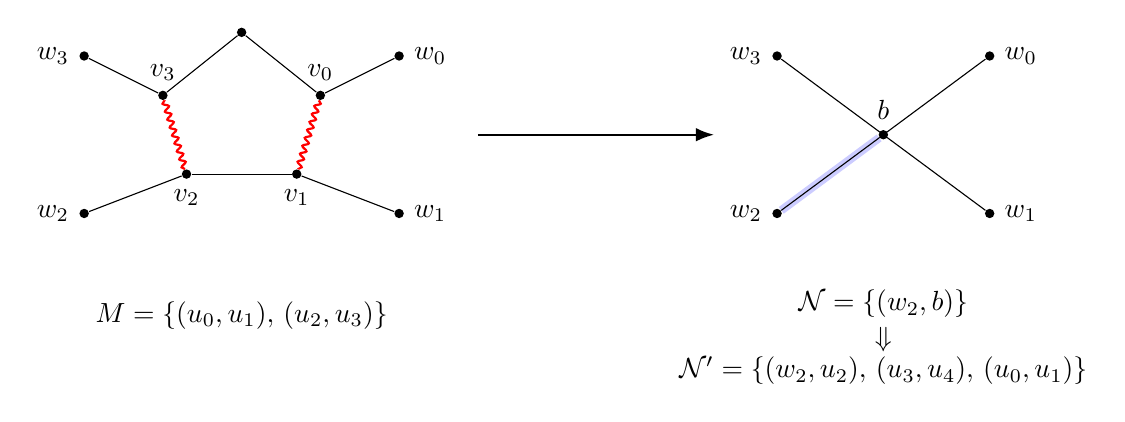
\begin{tikzpicture}

		% Left graph
		\node[fill=black, circle, inner sep=1.2pt, label=right:$w_0$] (w0) at (3,2) {};
		\node[fill=black, circle, inner sep=1.2pt, label=right:$w_1$] (w1) at (3,0) {};
		\node[fill=black, circle, inner sep=1.2pt, label=left:$w_2$] (w2) at (-1,0) {};
		\node[fill=black, circle, inner sep=1.2pt, label=left:$w_3$] (w3) at (-1,2) {};


		\node[fill=black, circle, inner sep=1.2pt] (v) at (1,2.3) {};
		\node[fill=black, circle, inner sep=1.2pt, label=above:$v_3$] (v3) at (0,1.5) {};
		\node[fill=black, circle, inner sep=1.2pt, label=below:$v_2$] (v2) at (0.3,0.5) {};
		\node[fill=black, circle, inner sep=1.2pt, label=below:$v_1$] (v1) at (1.7,0.5) {};
		\node[fill=black, circle, inner sep=1.2pt, label=above:$v_0$] (v0) at (2,1.5) {};

		% Edges
		\draw (v3) -- (v) -- (v0);
		\draw (v2) -- (v1);

		\draw (v3) -- (w3);
		\draw (v0) -- (w0);
		\draw (v1) -- (w1);
		\draw (v2) -- (w2);

		% Matching edges
		\draw[red, thick, decorate, decoration={snake, segment length=3pt, amplitude=1pt}] (v0) -- (v1);
		\draw[red, thick, decorate, decoration={snake, segment length=3pt, amplitude=1pt}] (v2) -- (v3);

		% Matching set label
		\node at (1,-1.3) {$M = \left\{ (u_0, u_1),\, (u_2, u_3) \right\}$};

		% Arrow to right side
		\draw[thick, -{Latex}] (4,1) -- (7,1);

		% Right graph (contracted blossom)
		\begin{scope}[shift={(1.5,0)}]
			\node[fill=black, circle, inner sep=1.2pt, label=above:$b$] (b) at (7.65, 1) {};
			\node[fill=black, circle, inner sep=1.2pt, label=right:$w_0$] (rw0) at (9,2) {};
			\node[fill=black, circle, inner sep=1.2pt, label=right:$w_1$] (rw1) at (9,0) {};
			\node[fill=black, circle, inner sep=1.2pt, label=left:$w_2$] (rw2) at (6.3,0) {};
			\node[fill=black, circle, inner sep=1.2pt, label=left:$w_3$] (rw3) at (6.3,2) {};
			\node at (7.65, -1.15) {$\mathcal{N} = \left\{ (w_2, b) \right\}$};
			\node at (7.65, -1.6) {$\Downarrow$};
			\node at (7.65, -2) {
				$\mathcal{N}' = \left\{ (w_2, u_2),\, (u_3, u_4),\, (u_0, u_1) \right\}$
			};
		\end{scope}

		\draw (rw0) -- (rw2);
		\draw (rw1) -- (rw3);

		% Highlighted edge
		\draw[line width=3pt, blue!20] (b) -- (rw2);
		\draw (b) -- (rw2);

		% Set N and N'


	\end{tikzpicture}
\end{center}
$N'$ is not maximum matching. Since $\{(v_i,w_i)\mid i\in\{0,1,2,3\}\}$ is maximum matching.
\nt{The above is not contradicting the theorem since the blossom with respect to $N'$ is not the blossom with respect to $M$.}

\section{Algorithm for Maximum Matching}
Suppose we start with a matching $M$ in $G$. We mark all the exposed vertices to be even and keep all the other vertices unmarked at this point. Hence, initially all the vertices are marked even. Now we use the same algorithm for finding augmenting paths as in the case of bipartite graphs but with slight modifications. In the case of bipartite graphs at each iteration we created the $M$-alternating tree we went one level at a time. But in the case of general graphs we'll go two levels at a time. So at each iteration we start with a vertex which is labeled even. Let $u$ be a vertex labeled. Now for each neighbor $v$ of $u$:
\begin{enumerate}[label=Case \arabic*:, leftmargin=*, align=left]
	\item $v$ is unmarked. This implies $v$ is matched. Then mark $v$ as odd and $M(v)$ i.e. the vertex matched with $v$ as even and continue the algorithm.
	\item $v$ is marked, and it is in the same tree as $u$. Then we have a blossom $B$ with respect to $M$. We shrink the blossom $B$ and therefore, we have the matching $M/B$ in the graph $G/B$. Mark the shrunk vertex $v_b$ even and continue the algorithm in the graph $G/B$ with the matching $M/B$.

	      If we get an even cycle then we just ignore i.e. ignore any neighbor marked odd.
	\item $v$ is marked even, and it is in a different tree from $u$. Let $r_u$ and $r_v$ are the root exposed vertices in the tree of $u$ or $v$ respectively. Then consider the path $P:r_u\rightsquigarrow u\to v\rightsquigarrow r_v$. This is an augmenting path from $r_u$ to $r_v$. Hence, the algorithm found an augmenting path with respect to $M$. Now unshrink the blossoms in $P$ to get the alternating path in $G$. Let that path is $\hat{P}$. So the algorithm updates the matching $M$ to $M\oplus \hat{P}$, and then we will start the algorithm again with the new matching $M\oplus \hat{P}$.

	      \begin{center}
		      \usetikzlibrary{arrows.meta, calc, decorations.pathreplacing}
		      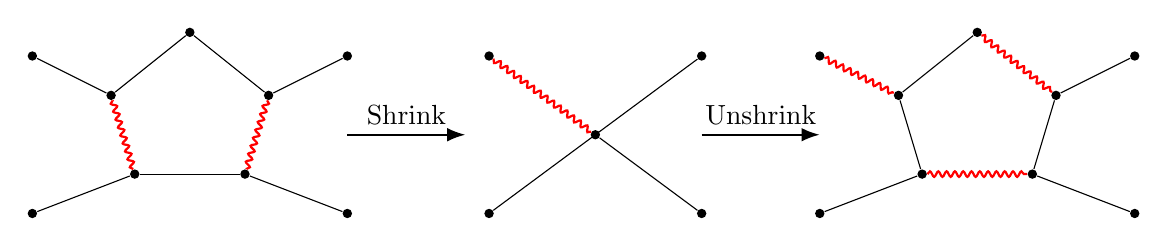
\begin{tikzpicture}

			      % Left graph
			      \node[fill=black, circle, inner sep=1.2pt] (w0) at (3,2) {};
			      \node[fill=black, circle, inner sep=1.2pt] (w1) at (3,0) {};
			      \node[fill=black, circle, inner sep=1.2pt] (w2) at (-1,0) {};
			      \node[fill=black, circle, inner sep=1.2pt] (w3) at (-1,2) {};


			      \node[fill=black, circle, inner sep=1.2pt] (v) at (1,2.3) {};
			      \node[fill=black, circle, inner sep=1.2pt] (v3) at (0,1.5) {};
			      \node[fill=black, circle, inner sep=1.2pt] (v2) at (0.3,0.5) {};
			      \node[fill=black, circle, inner sep=1.2pt] (v1) at (1.7,0.5) {};
			      \node[fill=black, circle, inner sep=1.2pt] (v0) at (2,1.5) {};

			      % Edges
			      \draw (v3) -- (v) -- (v0);
			      \draw (v2) -- (v1);

			      \draw (v3) -- (w3);
			      \draw (v0) -- (w0);
			      \draw (v1) -- (w1);
			      \draw (v2) -- (w2);

			      % Matching edges
			      \draw[red, thick, decorate, decoration={snake, segment length=3pt, amplitude=1pt}] (v0) -- (v1);
			      \draw[red, thick, decorate, decoration={snake, segment length=3pt, amplitude=1pt}] (v2) -- (v3);

			      % Arrow to right side
			      \draw[thick, -{Latex}] (3,1) -- (4.5,1) node[midway, above] {Shrink};

			      % Right graph (contracted blossom)
			      \begin{scope}[shift={(-1.5,0)}]
				      \node[fill=black, circle, inner sep=1.2pt] (b) at (7.65, 1) {};
				      \node[fill=black, circle, inner sep=1.2pt] (rw0) at (9,2) {};
				      \node[fill=black, circle, inner sep=1.2pt] (rw1) at (9,0) {};
				      \node[fill=black, circle, inner sep=1.2pt] (rw2) at (6.3,0) {};
				      \node[fill=black, circle, inner sep=1.2pt] (rw3) at (6.3,2) {};

			      \end{scope}

			      \draw (rw0) -- (rw2);
			      \draw (rw1) -- (b);

			      % Highlighted edge
			      \draw[red, thick, decorate, decoration={snake, segment length=3pt, amplitude=1pt}] (b) -- (rw3);

			      % Set N and N'
			      \begin{scope}[shift={(10,0)}]
				      \node[fill=black, circle, inner sep=1.2pt] (w0) at (3,2) {};
				      \node[fill=black, circle, inner sep=1.2pt] (w1) at (3,0) {};
				      \node[fill=black, circle, inner sep=1.2pt] (w2) at (-1,0) {};
				      \node[fill=black, circle, inner sep=1.2pt] (w3) at (-1,2) {};


				      \node[fill=black, circle, inner sep=1.2pt] (v) at (1,2.3) {};
				      \node[fill=black, circle, inner sep=1.2pt] (v3) at (0,1.5) {};
				      \node[fill=black, circle, inner sep=1.2pt] (v2) at (0.3,0.5) {};
				      \node[fill=black, circle, inner sep=1.2pt] (v1) at (1.7,0.5) {};
				      \node[fill=black, circle, inner sep=1.2pt] (v0) at (2,1.5) {};

				      % Edges
				      \draw (v3) -- (v);
				      \draw (v3) -- (v2);
				      \draw (v0) -- (v1);
				      \draw (v0) -- (w0);
				      \draw (v1) -- (w1);
				      \draw (v2) -- (w2);
				      \draw[red, thick, decorate, decoration={snake, segment length=3pt, amplitude=1pt}] (w3) -- (v3);
				      \draw[red, thick, decorate, decoration={snake, segment length=3pt, amplitude=1pt}] (v) -- (v0);
				      \draw[red, thick, decorate, decoration={snake, segment length=3pt, amplitude=1pt}] (v2) -- (v1);
			      \end{scope}
			      \draw[thick, -{Latex}] (7.5,1) -- (9,1) node[midway, above] {Unshrink};
		      \end{tikzpicture}
	      \end{center}
\end{enumerate}
\parinf

\textbf{Time Complexity:} The algorithm performs at most $n$ augmentations. Between two augmentations, it will shrink a blossom at most $\frac{n}{2}$ times as each shrinking reduces the number of vertices by at least $2$. The time to construct the alternating tree is at most $O(n+m)$. Hence, the total time taken by the algorithm is $O(n^2(n+m))=O(n^2m)$. \parinn
\section{Tutte-Berge Theorem}
\begin{Theorem}{}{tutte-berge-weak}
	In any graph $G=(V,E)$ for any matching $M$ in $G$ and any $S\subseteq V$, $$|M|\leq\frac{|V|+|S|-\emph{Odd}(G-S)}2$$ where $\emph{Odd}(G-S)$ is the number of odd components in $G-S$.
\end{Theorem}
\begin{proof}
	If $|S|>\emph{Odd}(G-S)$ then we already have this since $|M|\leq\frac{|V|}{2}$. So let $|S|\leq \emph{Odd}(G-S)$. Now each odd size component has at least one vertex unmatched in that component. So if that vertex is matched it is matched with a vertex in $S$. So $M$ leaves at least $\emph{Odd}(G-S)-|S|$ vertices unmatched. Hence, at most all the rest $|V|-(\emph{Odd}(G-S)-|S|)$ vertices are matched in $G$. Therefore, $|M|\leq\frac{|V|+|S|-\emph{Odd}(G-S)}2$.
\end{proof}

Now the algorithm stops if none of the cases 1, 2, or 3 happens. Let $G'=(V',E')$ is the final graph after shrinking all the blossoms algorithm encountered in its runtime. And let $M'$ is the matching in $G'$ after the algorithm stops. Now we will show that $M'$ is a maximum matching in $G'$.
\begin{lemma}{}{}
	When none of the 3 cases holds the matching $M'$ is maximum in $G'$.
\end{lemma}
\begin{proof}
	We will show that $M'$ attains equality in \thmref{tutte-berge-weak} for some subset $S$ of vertices. Since the algorithm stops the $M'$-alternating tree in $G'$ has no blossoms. So the $M'$-alternating tree is a forest. The algorithm marked the vertices of $G'$ as even or odd. Take $S$ be the set of all odd marked vertices. Hence, all the components of $G'-S$ are odd components where each component contains single vertex which is labeled even. So $\textsc{Odd}(G-S)=|V'|-|S|$. Therefore, $\frac{|V'|+|S|-\emph{Odd}(G-S)}2=\frac{|V'|+S|-(|V|-|S|)}2=|S|$. Since all the odd vertices are matched with even vertices in $G'$  we have $|S|=|M'|$. Hence, $|M'|=\frac{|V|+|S|-\emph{Odd}(G-S)}2$. Therefore, $M'$ is a maximum matching in $G'$.
\end{proof}
Let the algorithm performs $k$ blossom shrinking. Let $B_1,\dots, B_k$ are the blossoms. And let $M_i$ be the corresponding matching. $i=0$ corresponds to the original graph. Let $G_i=(V_i,E_i)$ be the graph after $i^{th}$ blossom shrinking. So $G_0=G$ and $G_k$ is the final graph after the algorithm stops. The above lemma shows that $M_k$ is a maximum matching in $G_k$. We will show that if we unshrink the blossoms one at a time in the reverse order of shrinking then we will get a maximum matching.
\begin{lemma}{}{}
	If $M_{k}$ is a maximum matching in $G_k$. Then $M_{k-1}$ is a maximum matching in $G_{k-1}$.
\end{lemma}
\begin{proof}
	$G_k$ is obtained from $G_{k-1}$ by shrinking the blossom $B_k$. So $G_k=G_{k-1}/B_{k}$, $M_k=M_{k-1}/B_k$. So $|V_{k-1}|=|V_k|+|B_k|-1$ and $|M_{k-1}|=|M_k|+\frac12(|B_k|-1)$. Let $S$ be the set of odd vertices in $G_k$. Now while unshrinking the blossom $B_k$  we add an even number of vertices ($|B_k|-1$) to one of the connected components to one of the connected components of $G_k-S$ and all these vertices are marked even. So the set of odd vertices of $G_{k-1}$ are the same as set of odd vertices in $G_k$. Hence, $\emph{Odd}(G_k-S)=\emph{Odd}(G_{k-1}-S)$. Therefore, $$\frac{|V_{k-1}|+|S|-\emph{Odd}(G_{k-1}-S)}2=\frac{|V_k|+|B_k|-1+|S|-\emph{Odd}(G_{k}-S)}2=|M_k|+\frac{|B_k|-1}2=|M_{k-1}|$$Therefore $M_{k-1}$ is a maximum matching in $G_{k-1}$.
\end{proof}Using the same $S$ we can show that if $M_{i+1}$ is a maximum matching in $G_{i+1}$ then $M_i$ is a maximum matching in $G_i$. Hence, we can conclude that if $M_k$ is a maximum matching in $G_k$ then $M_0$ is a maximum matching in $G$. Therefore, after unshrinking all the blossoms in the reverse order of shrinking we get a maximum matching in $G$. Therefore, the above algorithm returns a maximum matching of $G$.

Also, we have shown that the maximum matching attains equality in \thmref{tutte-berge-weak} for the set of odd vertices $S$. Hence, we have the following theorem.
\begin{Theorem}{Tutte-Berge Theorem}{tutte-berge}
	For any graph $G=(V,E)$, $$\max\limits_{M\text{ matching in }G}|M|=\min\limits_{S\subseteq V}\frac{|V|+|S|-\emph{Odd}(G-S)}2$$
	where $\emph{Odd}(G-S)$ is the number of odd components in $G-S$.
\end{Theorem}
Now from the Tutte-Berge Theorem we conclude that a graph has a perfect matching if and only if for every $S\subseteq V$, the number of odd components in $G-S$ is at most $|S|$. Hence, we have the following corollary.
\cor[]{Tutte's Matching Theorem}{For any graph $G=(V,E)$, $G$ has a perfect matching if and only if for every $S\subseteq V$, $\emph{Odd}(G-S)\leq |S|$.}